% This example An LaTeX document showing how to use the l3proj class to
% write your report. Use pdflatex and bibtex to process the file, creating
% a PDF file as output (there is no need to use dvips when using pdflatex).
\documentclass{l3proj}
\begin{document}
\title{Global Rugby Network FanZone (Web)}
\author{Ruxandra Bob \\
		Marios Constantinou \\
        Daniel Juranec \\
        Arnas Kapustinskas \\
        Andrew McCluskey}
\date{10 February 2017}
\maketitle
\begin{abstract}
Report on Team Project 3 coursework for Group V. The GRN Fanzone is a
 fan engagement web application developed to interface with the Global Rugby
 Network's online platform. The project tried to utilise 
 emerging technologies ranging from Angular to Firebase, and use
 cutting-edge methodologies, such as Test Driven Development and Agile
 project management. This report covers some of the considerations taken
 during development and explains some of the benefits and disadvantages
 of the way the development team operated.
\end{abstract}
%% Comment out this line if you do not wish to give consent for your
%% work to be distributed in electronic format.
\educationalconsent
\newpage
%==============================================================================
\section{Introduction}
This paper presents a case study of the project and software development process of Group V, which consists of five students studying Software Engineering at the University of Glasgow, done as part of the University's Team Project 3 course.
Our customers for the project were Global Rugby Network (GRN), who tasked us with creating a web application that would allow professional and amateur rugby clubs, teams, and players to interact with rugby fans. This social platform would then be integrated with the software that GRN already provides to rugby clubs. The end result is GRNFanZone, a fully functioning web application that allows people to follow their favourite clubs, see the latest posts made by them, find rugby matches happening near them, and much more.
The purpose of this document is to reflect on the achievements and challenges that arose during the development of this project. It also explores the concepts and methodologies touched upon in the concurrently running Professional Software Development (PSD) course, how we decided to implement them, and the effectiveness of our implementation.
The rest of the case study is structured as follows. 
Section \ref{sec:background} presents the background of the case study discussed, describing the customer and project context, aims and objectives and project state at the time of writing.
Section \ref{sec:cicd} discusses the Continuous Integration and Continuous Deployment techniques that were used in order to ensure higher quality of code and to continuously deliver new implementations. It also outlines challenges the team faced when using these techniques.
Section \ref{sec:frontend} talks about the key technology used for the Frontend implementation of the project. It contains an overview of the technology and justification for its usage in the project.
Section \ref{sec:conclusion} is the conclusion, where we evaluate our performance over the whole process, what has been learned from it and how this experience can benefit us in following professional software projects.
%==============================================================================
\section{Case Study Background}
\label{sec:background}
Include details of
\begin{itemize}
\item The customer organisation and background.
\item The rationale and initial objectives for the project.
\item The final software was delivered for the customer.
\end{itemize}
%==============================================================================
%\section{Alice}
%\label{sec:alice}
%\begin{figure}
\begin{center}

\includegraphics[width=7cm]{figures/alice}
\end{center}
\caption{Behind it was a little door}
\label{fig:alice}
\end{figure}
%==============================================================================
\newpage
\section{Continuous Integration and Continuous Deployment Considerations}
\label{sec:cicd}

The project used a multitude of Continuous Integration (CI) and Continuous
 Deployment (sometimes Delivery) (CD) techniques. A CI server's purpose "is to check the code
 repository for changes, check out the code if it spots any [changes], and run a
 list of commands to trigger the build."\cite{meyer2014continuous} A build is "ideally more than just
 compiling - it should also include a thorough test suite to help verify that the code
 still works with every change."\cite{meyer2014continuous} This gives a development
 team a quick, automated way of checking their code works, follows a style guide and
 doesn't break any other work. 
 
One of the key concepts of CI is often phrased as: "Commit Daily, 
 Commit Often"\cite{meyer2014continuous}. For our project, this was sometimes a struggle. 
 This was due to a small number of factors, which boiled down to: "We don't work on the project 
 every day", and "I'm not used to git". There was little we could do to remedy the former issue - 
 all we could do was commit often \textit{whilst we worked on the project}. The gitflow 
 branching system we used in the VCS (see section \ref{sec:VCS}) was unfamiliar to several 
 members of the team, and it took time for everyone to become accustomed to the system. As the
 project progressed however, more builds were made, more commits pushed, and more bugs found.

Another hurdle at which we fell was getting into the habit of writing tests for our code. I shall 
 mention this briefly here, but for more details please see section \ref{sec:testing}. In Fowler's 
 2006 paper on CI, he says: "Imperfect tests, run frequently, are much better than perfect tests 
 that are never written at all."\cite{fowler2006continuous}
 
Continuous Deployment is the practice of continually deploying working builds to production
 as often as possible. It adheres to the Agile principles of:
 \begin{itemize}
 \item
 Our highest priority is to satisfy the customer
 through early and continuous delivery
 of valuable software. \cite{agileprinciples}
 \item 
 Deliver working software frequently, from a 
 couple of weeks to a couple of months, with a 
 preference to the shorter timescale. \cite{agileprinciples}
 \end{itemize}
 In our project, as soon as a new feature is merged into the dev branch,
 tests are run, and then the changes are deployed to a staging server, hosted by firebase. Similarly,
 as soon as dev is merged into master, master is pushed to our production server, also hosted by Firebase.
 The dev branch was typically merged into master once a week, allowing time for any changes to be made 
 to features that weren't quite perfect, and to iron out any bugs that were found after time in dev.
 
Our CI and CD was operated using Gitlab's integrated CI system. This uses docker to
 run a set of instructions defined in the 'gitlab-ci.yml' file.  Instructions are 
 separated into tasks. Tasks belong to stages - in our project, these were
 "test" and "deploy". The tasks are run as builds within a pipeline. The docker instances were
 in some cases hosted for free by Gitlab (sponsored by a cloud company). In other cases,
 builds were run on team computers. A common upper limit for build time is quoted as 
 10 minutes\cite{fowler2006continuous} - ours typically ranged from 5-15 minutes, with some exceptions that were 
 typically waiting on the gitlab CI runners to free up. The single largest time-drain was
 running \texttt{npm install} every time docker span up a new instance. Running tests typically took under
 a minute after this.
 
 \begin{figure}[H]
\begin{center}
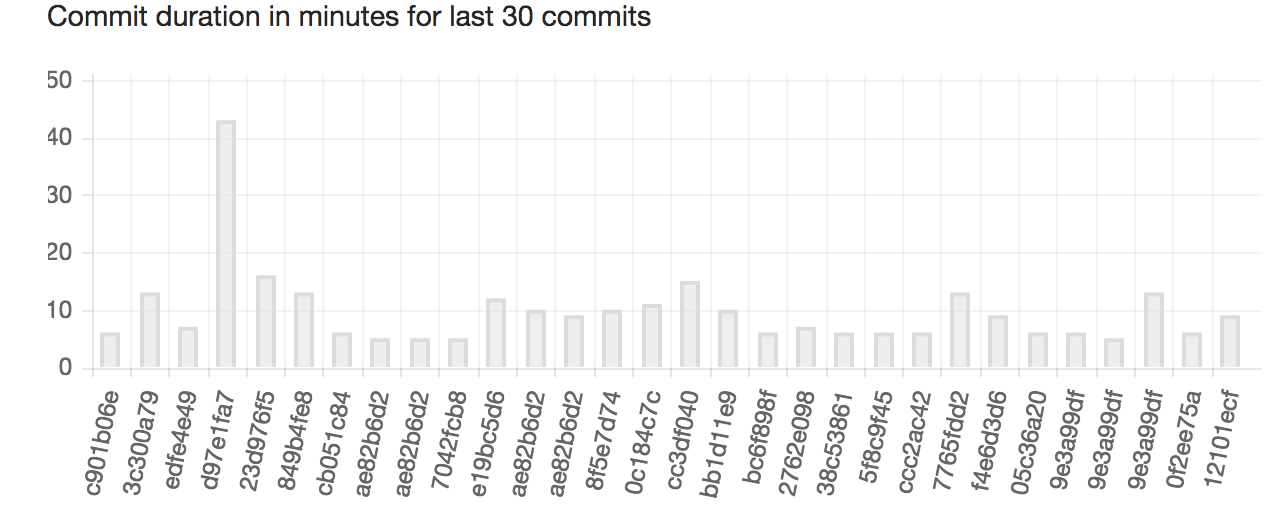
\includegraphics[width=9cm]{figures/cicd_build_duration}
\end{center}
\caption{Build Duration for last 30 commits from 21:28 on 19/03/2017}
\label{fig:cicd_build_duration}
\end{figure}



% Describe Linting task
The first task used by the project's 'test' stage ran a series of lint checks over the 
 project's source code. Linting involves performing static analysis on code to detect bugs 
 or violations of a style guide. These kind of checks are also performed by compilers and 
 so on. These issues can range from missing semicolons, to using a mix of 
 double and single quotes, to whether a function is never called. The task tested CSS, 
 JSON, typescript, javascript,  HTML and LESS. Whilst this was often annoying, these tests 
 did help maintain a higher quality of code in the codebase. As our policy was to not allow a 
 merge to dev take place if a branch was not passing tests, we had a method of 
 enforcing that the standards we defined were upheld.

% Describe testing task
The second task ran the project's tests. Again, this task had to complete successfully in 
 order for a branch to be merged into dev. This stage also generated coverage reports which 
 were used to give the team an indication of how well our code was tested.
 
 \begin{figure}[H]
\begin{center}
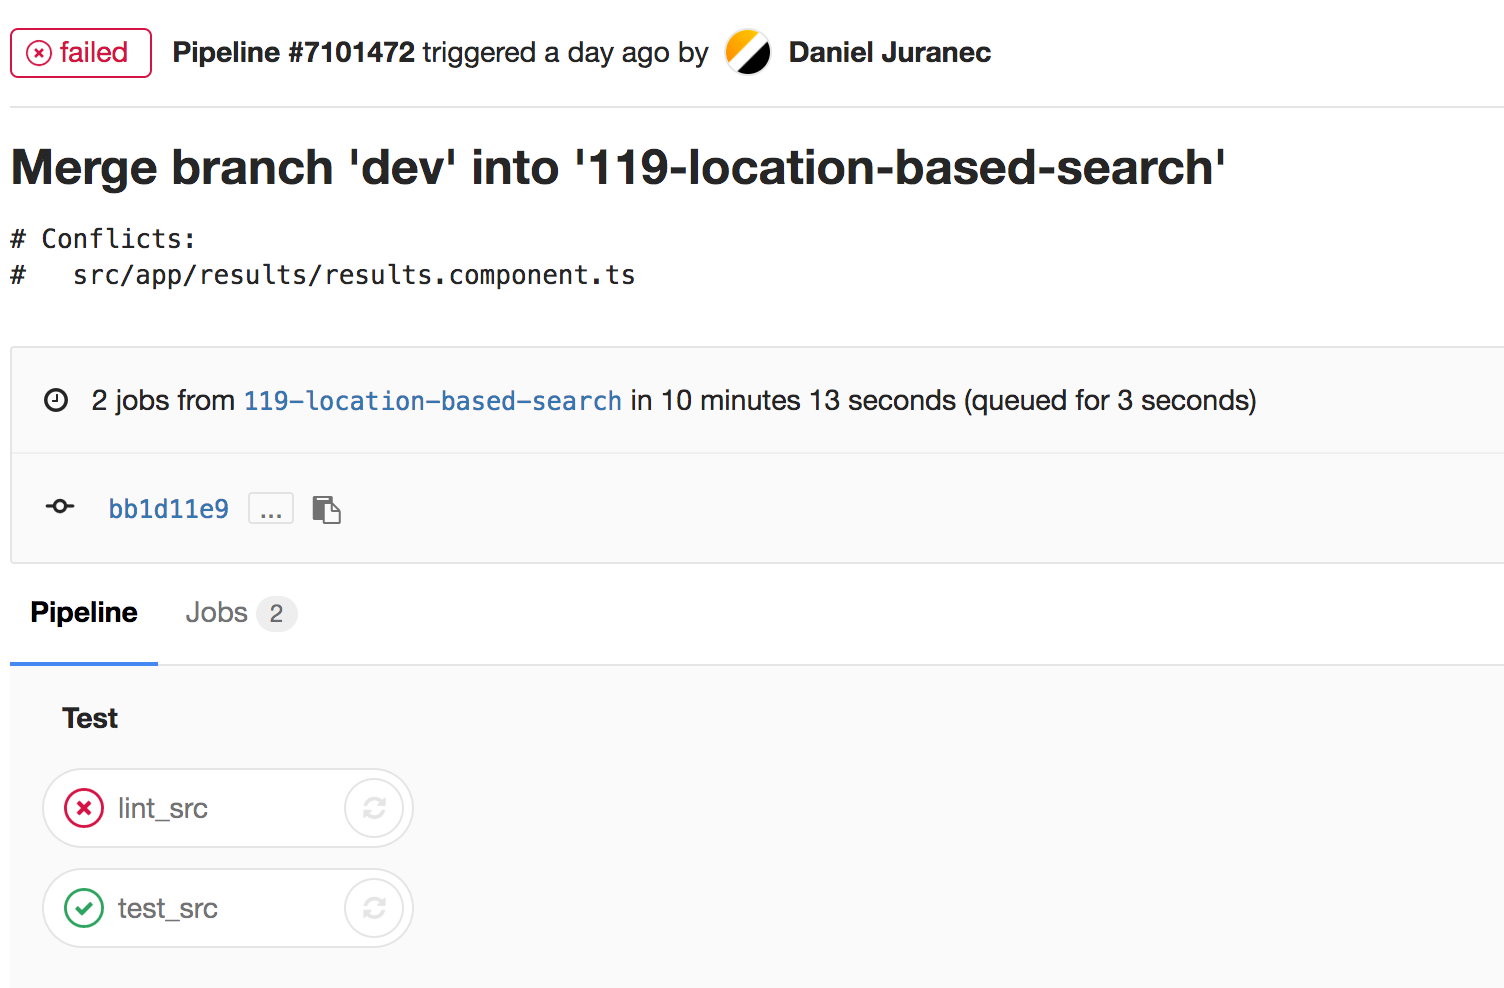
\includegraphics[width=9cm]{figures/cicd_failed_pipeline}
\end{center}
\caption{Example of a failed pipeline in GitLab}
\label{fig:cicd_failed_pipeline}
\end{figure}

 
% Considered combining test tasks
Merging these two tasks was considered, but left aside for now. The tasks take 5-10 minutes 
 each to run, and are run in parallel. The downside of this separation is the fact that \texttt{npm install} 
 is run twice. However, by leaving the tasks separate, we get a quicker, clearer indication
 of which part of the stage failed - actual functionality, or a style issue.

 \begin{figure}
\begin{center}
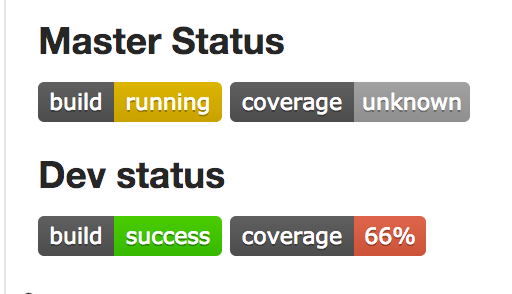
\includegraphics[width=4cm]{figures/cicd_coverage_buttons}
\end{center}
\caption{The buttons used to display pipeline status and test coverage}
\label{fig:cicd_coverage_buttons}
\end{figure}

% Describe deployment tasks
The Continuous deployment tasks were both essentially the same, but related to which branch was being 
 committed to. As both dev and master can only be merged into instead of committed to, these tasks can 
 be run only on merge commits to dev or master. The tasks run tests (to allow coverage reports for the branches) 
 and then deploy to our live servers. The dev branch deploys to the staging zone, and 
 master to our production site. 
 
The fact that this is automated helps encourage rapid deployment, as the steps take some time, and are 
 boring for people to do. This methodology takes out the human steps, and means that the development team 
 can focus on development. These rapid deployments also help by making it easy for the team to demonstrate 
 and generate feedback from the public.


% consider how it helped us and how it could have been improved
The CI and CD processes helped us by keeping our code of high quality, preventing broken commits and reducing 
 manual time spent doing menial tasks. However, it took a fairly large period of time to get working and to
 optimise into time chunks that were consistent with the goal of 10 minutes. It is arguable that the time 
 could have been better spent working on the actual project itself. As a counterpoint to this, it could be
 argued that the CI and CD has saved the development team time in fixing bugs later on, and by ensuring code is more
 readable, reducing time wasted understanding the code.

%==============================================================================
\newpage
\section{Frontend Technology Considerations}
\label{sec:frontend}

At the start of the project, GRN chose to give us a set of technologies they 
 wanted us to use. These included defining Angular 2 as our frontend framework.
 Angular is a framework maintained by google, which has been gaining popularity
 over the last 8 years\cite{angularjsoverview}. The framework uses typescript, 
 a type safe flavour of javascript. It focuses on being portable, high performance
 and easy to write\cite{angular_features}. Many of the contributors to Angular are from Google, but 
 the project is open source under the MIT license and anyone can commit to 
 it\cite{angularjsoverview}. Angular is built on top of NodeJS, providing 
 easy access to a wide range of external components.
 
Angular embeds code in html, and uses a "controller" to define component behaviour. This
 "component" object is the basis of most Angular development. Angular also tries 
 to minimise the logic in controllers, by either abstracting it to other components
 or building "services" - shared libraries of code snippets. The final piece of the puzzle
 is a "module" which co-ordinates resource injection into controllers from one 
 file. A project may have more than one module for it's subsections, but we stuck to
 one file. We made use of several services, and many components.
  
 % Pros and cons of ng-cli
Angular provides a CLI that makes it easy to start projects, and provides 
 templates for components, services and modules. This allows a "quick start"
 option. The basis of the project was generated in under a minute, which set up
 testing frameworks, a basic starter app and a \texttt{package.json} file for NPM.
 When generating a new component, a html template, CSS styles file, karma 
 jasmine test file as well as the typescript controller. These were populated
 with template code to allow easy starts. This helped ensure we could get to 
 the business logic of the component or service quickly, without wasting time 
 on the configurational nightmare javascript and typescript development has
 become.
  
 \begin{figure}[H]
\begin{center}
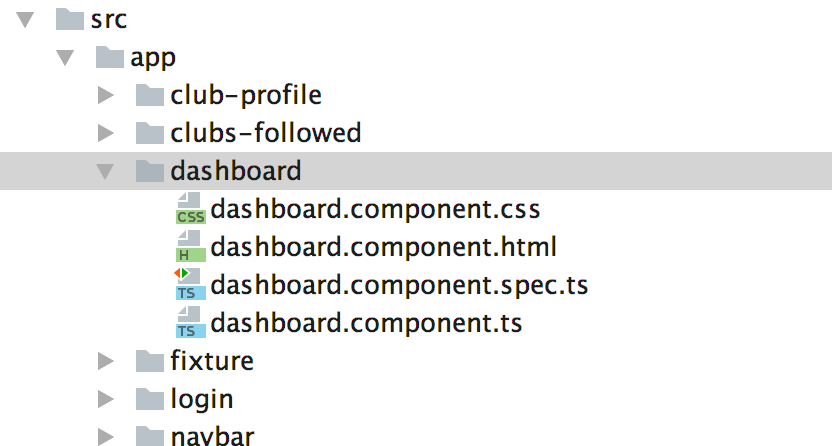
\includegraphics[width=7cm]{figures/frontend_components}
\end{center}
\caption{A selection of components used in the GRNFanzone}
\label{fig:frontend_components}
\end{figure}
   
  
 % Why we liked it (easy to maintain, works out the box, good documentation)
Angular gave us a huge advantage when working on this project. Components provide
 an easy way of separating concerns, and reducing code duplication. Generating new
 code is easy with the CLI, and entire projects can be started off and be running
 in hours. The documentation for Angular is also excellent. Maintained by google,
 it is kept up-to-date with the regular releases Angular receives.
 
 % why we disliked it (steep learning curve) 
The most significant barrier to using Angular was our own inexperience. 
 Thus far, our formal education has not involved developing webapps in
 javascript based frameworks. Beyond this, typescript was new to every
 member of the team. This meant that there was a steep learning curve for
 the team to deal with and adapt to. This caused some issues early on, 
 before we had a good grasp of how to use the actual features Angular
 provides.
 
 % How easy it was to test
One of Angular's benefits is that its developers have thoughtfully
 considered testing. Software testing has long been an important
 aspect of software development, and this has only become more true
 in recent years \cite{tuteja2012testing}. The Angular CLI generates
 a functional karma file, which has been configured for Angular. The
 Angular CLI also provides an interface for running tests. Parameters 
 range from single/constant runs of the test suite to enabling code
 coverage reporting. In spite of this, it was found to be very 
 difficult to mock our services which used angularfire to generate
 good tests (please see section \ref{sec:testing} for more on this).
 
\begin{figure}[H]
\begin{center}
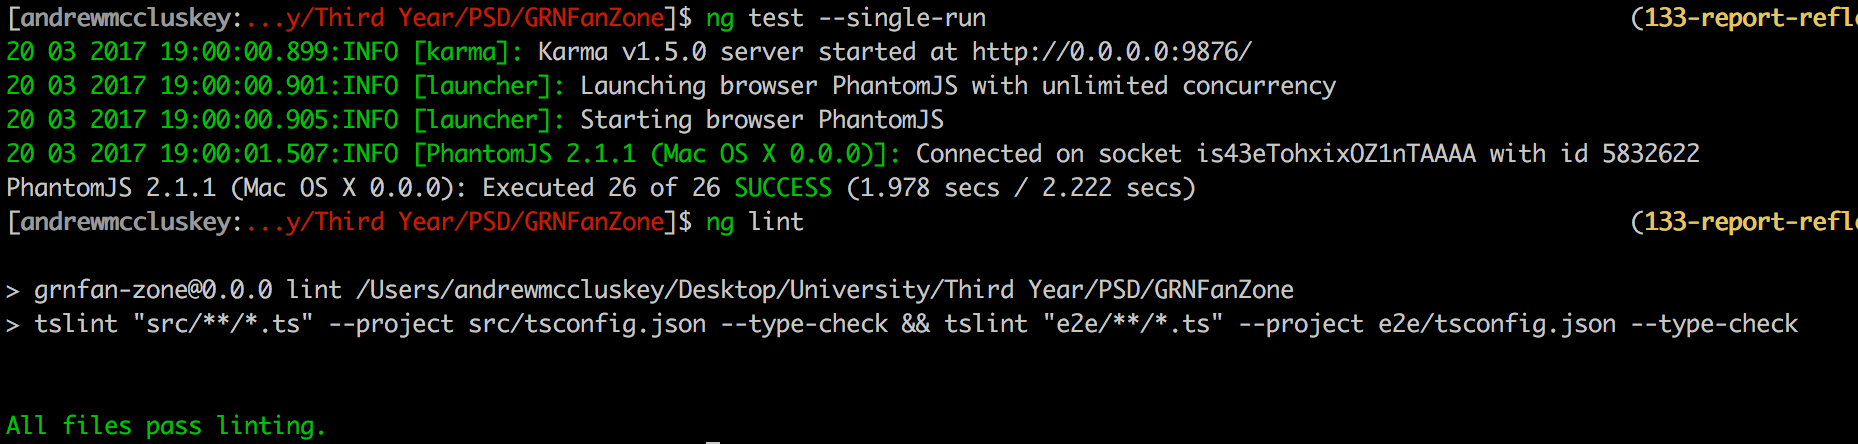
\includegraphics[width=11cm]{figures/frontend_ng_cli}
\end{center}
\caption{Using the Angular CLI to run tests and linting}
\label{fig:frontend_ng_cli}
\end{figure}


%==============================================================================
\newpage
\section{Project Planning}
\label{sec:planning}

After the project allocation day, GRN have sent us a project brief containing greater details about the project itself, as well as a list of functional requirements that the final product would be expected to meet. The first task we needed to complete was a detailed requirements document, that would contain non-functional and any additional functional requirements. It was decided that the focus of the first month would be allocated to finalizing the document, in order to assure that the client approved of the direction the team decided to take in working on the project.

As part of the requirements gathering process, the team developed four personas and an epic description of how they would end up using the FanZone in their daily lives, illustrating that by documenting epic user stories. This was followed by writing down user stories centered around the following entities: team manager, sponsor, player, club supporter, rugby fan and international rugby fan. Doing this eased the process of identifying useful requirements and helped the team visualize what the final product should be offering potential users.

After the initial requirements were outlined, the team followed by designing wireframes of the web application. Initially, each team member delivered a pencil-drawn sketch of each expected application screen. Afterwards, the best design from each wireframe were merged into the main wireframes, drawn using draw.io. GRN warned us that the main wireframes would not offer useful guidance when thinking how the application should transition to a mobile format, so the team repeated the process to generate mobile wireframes.

Over the weeks dedicated to producing the requirements document, the team kept close contact with GRN, who have repeatedly offered helpful feedback and guidance regarding how the team can meet their expectations of the final product. This gave us some understanding of what the client found to be of most importance, and it helped us in the next stage in our project, which was prioritising the features of the application and separating them into achievable goals for each iteration.

There were several aspects to be taken into consideration while deciding on a concrete structure of the development process. We had to consider our lack of experience with the technologies to be used and the fact that the available time to work on the project would vary as the academic year progressed. Another thing to consider was the fact that due to the agile methodology we decided to follow, at the end of each iteration, the product needed to be functional. Thus, it was decided to settle on having smaller, more easily achievable goals in the beginning, which would incrementally become more complex as advanced. In the end, we settled on seven iterations, excluding the initial one focused on the requirements document.


The goals for each iteration become increasingly challenging, based on the expectancy that the first one or two iterations would offer all team members some hands on experience with both Angular2 and Firebase. The goals for each iteration were the following: first iteration - login and sign up; second iteration - dashboard and followed pages; third iteration - post creation and management; fourth iteration - view and edit profile, posts on comments; fifth iteration - search for teams/clubs/players or fixtures; sixth iteration - translation and additional tasks; seventh iteration - additional features, refinement, documentation.

\begin{figure}
\begin{center}
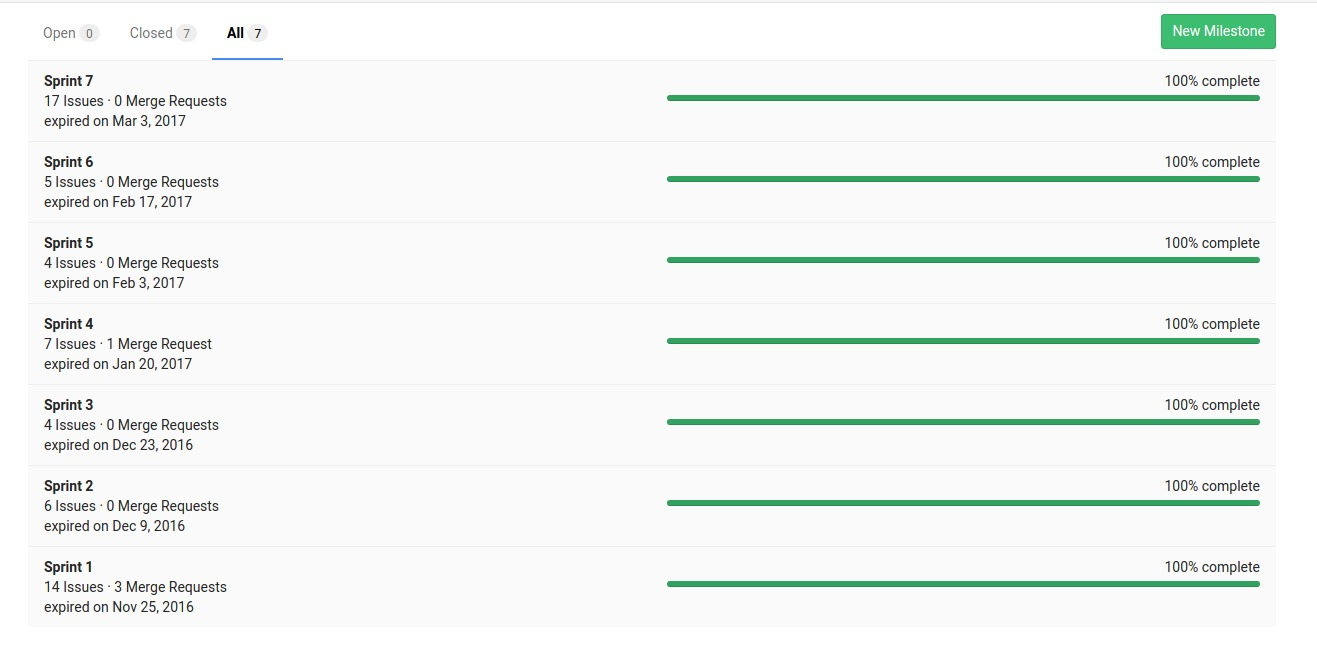
\includegraphics[width=15cm]{figures/milestones}
\end{center}
\caption{Project milestones}
\label{fig:project_milestones}
\end{figure}


Gitlab allowed us to create project milestones. Each of them had a number of issues associated with it, the issues consisting of the goals for the respective iteration split into several multiple smaller issues. The deadline of each iteration would also appear on each issues, becoming bright red as the date came nearer, in order to alert the person assigned to the task.

Throughout the project, our process was modified and improved by having team retrospectives around the end of each iteration. The format of the retrospectives consisted of every team member going through what they thought went good in our past iteration, what they thought went bad and what ideas they have to improve our workflow in future iterations. All these were discussed within the team and what the majority considered useful ideas were then included in the further development. The main points of each retrospective are documented on the wiki page of the project, which can be found on Gitlab.



%==============================================================================
\newpage
\section{Reflection on Agile Methodology}
\label{sec:agile}

% short description of agile development

Agile software development consists of a set of practices and methods derived from the principles described in the Agile Manifesto. Agile enforces a strong collaboration between the development team and the business stakeholders, self-organizing teams and frequent delivery of functioning software.\cite{agile_overview}

As agile development was highly recommended as part of our software development process, in the initial team meetings, we have decided to use the Scrum methodology.
 
 % short description of SCRUM
 Scrum is an agile framework originally formalized for software development projects. Scrum defines two major roles within a development team: the product owner and the scrum master. The product owner should maintain communication with the stakeholders and create a prioritized list goals to be achieved. The scrum master keeps the team focused and leads team meetings.\cite{scrum_overview}
 
 % our agile development
 Within our team, Andrew was the product owner and Ruxandra was the scrum master. After the first few team meetings, where the focus was on finalizing the initial requirements gathering, the focus was shifted to dividing the prioritised expected features. As a result of discussions between the product owner and the rest of the team, it was decided to split the work into seven sprints, each of them lasting two weeks. One sprint would end on Friday and the next one would start the following Monday. (Figure 6)
 
 
 It was decided that instead of daily scrums, the team would have two weekly meetings, one on Wednesdays, during the software development lab, and one on Fridays. The format of the meetings included everyone describing what they've worked on since the previous meeting and the work they plan on completing until the next meeting. Each team member also discussed any difficulties they encountered, how they overcame them or whether they feel that they need help with certain issues.
 
 The scrum master was tasked with closely observing these meetings. They had to determine whether the team could handle the workload of the respective sprint, if everyone in the team had something to work on and how to efficiently assign members to assist those who need help with something. The scrum master would also take into consideration any complaints or suggestions from the rest of the team, as well as initiate team retrospectives at the end of each sprint.
 
 As the project progressed, our scrum process underwent a few changes. Once the desired goals and the predicted timelines were better defined, it was decided that one meeting during the PSD lab would be sufficient, with any additional meetings to be arranged if deemed necessary. Meanwhile, the team would communicate daily through a group chat on Facebook messenger, in order to keep everyone updated with the general progress.
 
 Towards the end of the first semester, our sprints needed quite a few adjustments, due to the increase in additional assignments from other courses, that everyone in the team had to complete. There was also a slight halt in communication during the winter break, as all team members went home for the holidays. However, the additional time left at the end of our initial schedule allowed us to maintain the initial seven sprints and just shift everything by a few weeks.
 
 As we became more comfortable working as a team and since at that point everyone was comfortable with the new technologies, team meetings became less structured and less formal. Along the way, the meetings became open discussions, while still making sure everyone is kept up to date. At the beginning of the second semester, our scrum framework transitioned into a less clearly defined agile framework, which still followed the main principles of the methodology. Sprints became of variable length (between one and three weeks) rather than a constant two weeks.
 
 \begin{figure}
\begin{center}
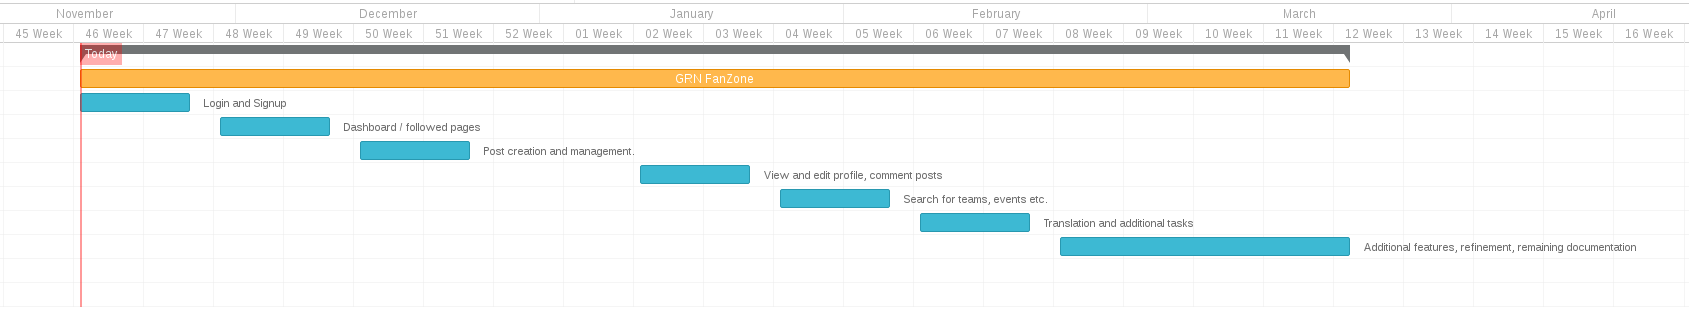
\includegraphics[width=15cm]{figures/agile}
\end{center}
\caption{Gnatt Chart for Development Process}
\label{fig:cicd_build_duration}
\end{figure}

 
 At the beginning of the development process, the product owner split every goal into separate small issues. The members of the team were also encouraged to make small commits as often as possible and only merge one small issue at a time in the development branch, in order to avoid disrupting someone else's work by generating conflicts. Every merge request needed to be approved by at least one more team member, in order to maintain the quality of the product.
 
 At the end of each sprint, the product was fully or almost fully functional with respect to the features that needed to be completed up to that point. The end of most sprints coincided with the customer meetings. Thus, we were able to receive almost immediate feedback from both GRN and supervisors. This also offered us the opportunity to make additional improvements in the short time left between sprints.
 
 To maintain the close communication with our client, as dictated by the agile methodology, the product owner would communicate weekly updates by email. The team was also in close contact with the development team of our client company, which was available for questions and pointed us towards useful resources. This was helpful in assuring that our version of the product would be as close as possible to the expectations of GRN, with respect to both design and implementation.
 
 
 
%==============================================================================
\newpage
\section{Conclusions}
\label{sec:conclusion}


Explain the wider lessons that you learned about software engineering,
based on the specific issues discussed in previous sections.  Reflect
on the extent to which these lessons could be generalised to other
types of software project.  Relate the wider lessons to others
reported in case studies in the software engineering literature.

%==============================================================================
\bibliographystyle{plain}
\bibliography{dissertation}
\end{document}
\grid

\grid
\grid
